\chapter{Paper II}\label{chap:paper2}
\section{Introduction}\label{sec:p2-intro}
In Paper II we deal with the velocity distribution of local stars which was discussed in the previous chapter. Specifically, we determine the velocity distribution and velocity moments of Solar neighbourhood white dwarfs (WDs) in Gaia EDR3. In order to do this we make use of the methods derived in \cite{dehnen:98a} and \cite{dehnen:98b} the first of which has not been employed for the \textit{Gaia} data prior. Since the method does not rely on any measurements of radial velocity the WDs are ideal candidates since they very rarely have such measurements available. 

The velocity distribution is a powerful tool to decode the evolution of the Milky Way's components, as the community has been able to show in the past few decades. Recent research has been able to show a staggering amount of substructure in the velocity distributions \citep{antoja:12, kushniruk:17, dr2:kinematics} where we can see individual velocity structure up to hundreds of km s$^{-1}$ away from Solar motion as well as horizontal arches in $(U, V)$ that span across the distribution. In addition to classical motions in $U, V, W$, the field has grown to include distributions in actions and angles, called orbit space (e.g., \citealt{trick:19, trick:21, trick:22}). In orbit space we can see clear ridges that are linked closely to the various structures in velocity space. Going forwards, both of these spaces will be important to understand the dynamical structure of the Milky Way.

The velocity distribution of WDs has, as mentioned, not been as easy to probe as that of the rest of the stars in the Solar neighbourhood. This leads to smaller samples which a couple of decades ago were only in the few hundreds \citep{sion:77, sion:88} and more recently samples which range from a couple of thousand to a few tens of thousands \citep{rowell:11, anguiano:17}. Recent works that investigate the kinematics of WDs are \cite{torres:19} who used Gaia to identify the \textit{Hercules} stream in the WDs and \cite{raddi:22} who determined the age-velocity dispersion relation of WDs. These samples are about as large as any that have been used, with {$\sim$}14\,000 and {$\sim$}3000 for the two papers respectively. In my second paper, our method provides us with a sample of 129 675 WDs, the largest to date. We use this sample to identify known substructure as well as some novel features in velocity space. In addition to this, we also manage to identify two kinematically separate WD populations, which are attributed to two parallel cooling sequences seen in the colour-magnitude diagram (CMD) of WDs and demonstrated in section \ref{sec:p2-whitedwarfs}. We tenatively linked this to recent star formation which, it has been suggested, matches the times of flybys of nearby dwarf galaxies \citep{ruiz-lara:20}. 

\section{White dwarfs}\label{sec:p2-whitedwarfs}
\begin{figure}[t!]
    \centering
    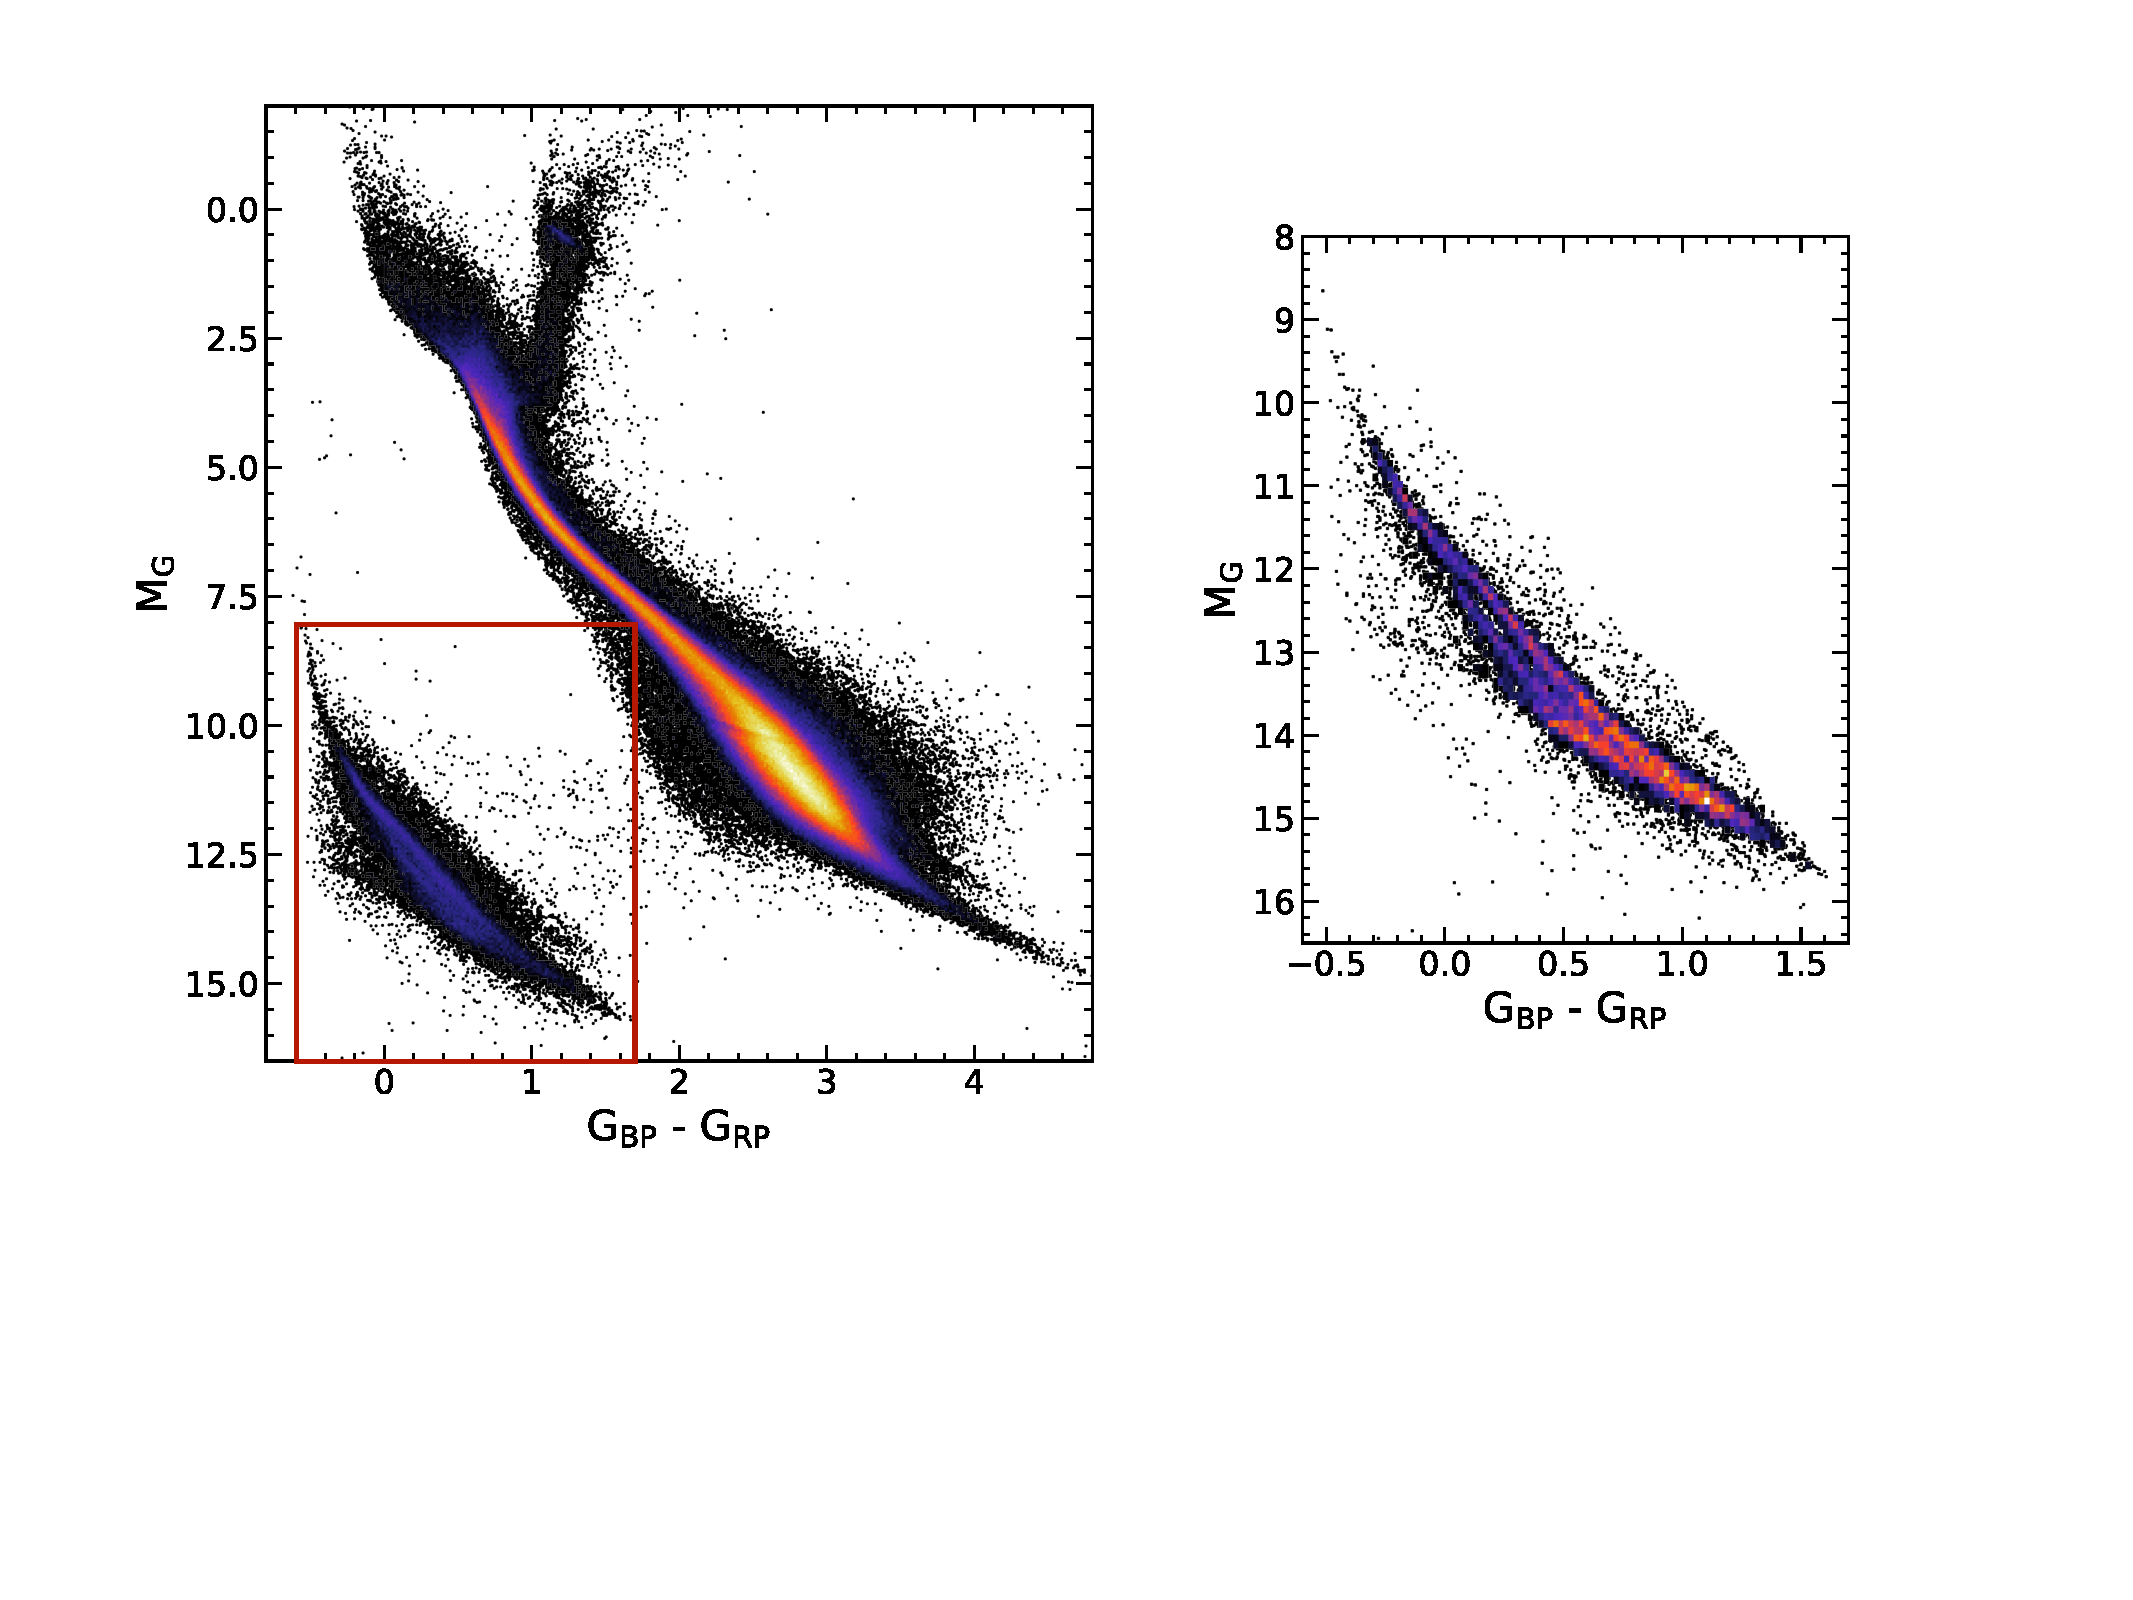
\includegraphics[width=0.95\textwidth]{images/gaiacmr.pdf}
    \caption{Colour-magnitude diagram of stars available as part of the Gaia data. Colour shows the square root of the number density. The left panel shows all stars in DR3 that are within 200 pc overlaid with a 500x500 histogram. The red box shows the WD region for which is then shown on the right in a similar style but for stars within 100pc and with increased bin width. A separation into two sequences can clearly be seen.} % Fig. 4.1
    \label{fig:cmd}
\end{figure}
Stars can be called `nuclear foundries', as they fuse hydrogen into helium, `shaping' metals from other metals through nuclear processes. This process creates outward thermal pressure which holds the star up against gravitational pressure in hydrostatic equilibrium. The hydrogen is not infinite and eventually runs out and the star contracts, shedding its outer layers while the core begins fusing helium into heavier elements, creating a planetary nebula around it. For massive stars, the core is large enough that many heavier elements can start fusing but for stars between about $0.6-10\ \mathrm{M}_\odot$, at some point this is insufficient and `electron degeneracy'\footnote{Electron degeneracy pressure and more is explained in \cite{kippenhahn:12}} occurs and provides the necessary outward pressure. The star no longer fuses and all that is left is the core, a stellar `corpse' called a white dwarf. This is the fate of 97\% of all stars in the Milky Way \citep{fontaine:01}. The WD will live for a long time, but cools slowly, growing fainter and redder over time which can be seen in the CMD of WDs, shown in Fig. \ref{fig:cmd}. The WD will be difficult to observe photometrically, as it is rather faint, and spectroscopically, due to the metals sinking below the observable photosphere as well as thermal broadening. 

Despite this, Gaia is able to observe quite a large number of WDs photometrically. In the Solar Neighbourhood (within 500 pc) we can, after some quality cuts, find about 130 000 WDs in EDR3. However, if we use an even closer sample limited to 100 pc, we can observe that the WD sequence is in fact not singular, but split into two. This result was first identified in \cite{dr2:hr} and has had two major suggestions put forth to explain it. Explanation \textbf{a)} suggests that the second sequence arises due to atmospheric differences in WDs. The upper, redder, sequence have hydrogen-dominated spectra (called DAs and constitutes {$\sim$}80\% of observed WDs) whereas the lower, bluer, sequence contains WDs with Helium (called DBs) or heavier elements dominating their atmospheres. We can refer to this simply as DAs or non-DAs for the purposes of Paper II. For a full descripion of spectral classes of WDs and their meaning, see table \ref{tab:p2-wds}\footnote{The `D' in the spectral classifications stands for degenerate.} This explanation has shown to be able to explain the CMD bifurcation very well in works like that of \cite{kilic:18, kilic:20} and \cite{gentile-fusilo:19}. Another recent discovery about the WDs is that their mass distribution is bimodal, with a main Gaussian centered on ${\sim}0.6\ \mathrm{M}_\odot$ and a secondary, smaller Gaussian around ${\sim}0.8\ \mathrm{M}_\odot$ (e.g., \citealt{elbadry:18, kilic:18, kilic:20}). This has lead to explanation \textbf{b)} that the second sequence could consist of heavier mass WDs, which have fainter and bluer cooling tracks. In single star evolution, the more massive WDs would come from more massive progenitors, which then become WDs much on shorter timescales. For this reason they would have colder kinematics due to the age-dispersion relation \citep{aumer:16}. Mergers were suggested as a source of massive WDs but was ruled out by \cite{kilic:20} who failed to discover significant massive WDs with hot kinematics. Instead \cite{elbadry:18} shows that with the right choice of initial-final mass relation and continuous star formation, the second sequence can be populated by late-forming WDs. In summary, the second sequence can be explained as massive WDs formed recently. 
\begin{table}[t!]
\caption{Spectral classification of white dwarfs. The name of the spectral class and its definition.}\label{tab:p2-wds}
\begin{tabular}{|c|r|}
\hline
\textbf{Spectral class} & \multicolumn{1}{c|}{\textbf{Definition}} \\ \hline
DA & Hydrogen dominated spectrum \\
DB & Helium dominated spectrum \\
DC & Continuous spectrum, featureless \\
DO & He II and He I or H features \\
DZ & Metal lines dominate spectrum \\
DQ & Carbon lines dominate spectrum \\\hline
\end{tabular}
\end{table}
The two scenarios can be distinguished by their kinematics. The atmospheric composition should not have any bearing on the kinematics while, as explained above, the mass of WDs does. Therefore, we can investigate the kinematics of the two populations and try to provide insight into the casue of the CMD bifurcation. 

\section{Inferring $f_v$}\label{sec:p2-inferring}
\begin{figure}[t]
    \centering
    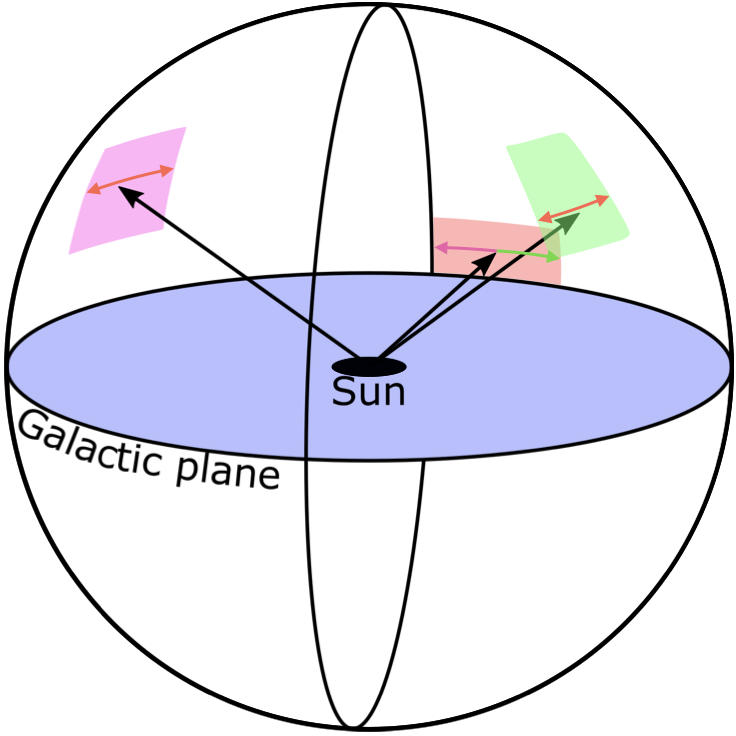
\includegraphics[width=0.45\textwidth]{images/projection.png}
    \caption{An illustration of positions on the celestial sphere from the point of view of a Solar system observer.} % Fig. 4.2
    \label{fig:projection}
\end{figure}
As shown in \cite{dehnen:98b}, the mean motion $\langle\bm{v}\rangle$ and velocity dispersion $\bm{\sigma}$ can be determined for a sample of stars given a few caveats. The on-sky positions have to be uncorrelated with the velocities, which means that we see the same velocity distribution regardless of where on the sky we look. Consider the regions shown in Fig. \ref{fig:projection}. If there is a general mean motion for all parts of the sky, the line-of-sight motion of the red region will be given by the tangential motion of either pink or green regions in the direction of the red region, shown here using red arrows on the pink/green regions. Conversely, the tangential motion components of red region that points to the left and right will give, approximately, the line-of-sight motion of the other two components, as indicated by the colouring of the arrows. 

The same concept was used for the even more impressive feat of inferring the velocity distribution of Hipparcos stars in \cite{dehnen:98a}. We can write the probability distribution of tangential or transverse velocities in a given direction $\hat{\bm{r}}$ as $\rho(\bm{q|\hat{\bm{r}}})$ where $\bm{q}$ is the 2D vector of tangential velocities. To relate this distribution to the full velocity distribution we can write
\begin{equation}
    \rho(\bm{q|\hat{\bm{r}}}) = \int \mathrm{d}v_r f(\bm{v}) = \int \mathrm{d}v_r f(\bm{p} + v_r\hat{\bm{r}}),
\end{equation}
where $\bm{p}$ is the 3D projection of the tangential motion. The true distribution can of course not be determined precisely using transverse motion alone but it can be estimated with a log-likelihood maximization of some model of it. We do this numerically by defining the velocity distribution to be
\begin{equation}
    f(\bm{v}) = e^{\phi(\bm{v})},
\end{equation}
where $\phi(\bm{v})$ is given on a 3D velocity grid with $L_U\times L_V\times L_W$ cells with widths $h_U\times h_V\times h_W$. The final expression for the function we seek to maximize, as a function of $\phi(\bm{v})$, is: 
\begin{equation}\label{eq:mple}
    \scalemath{0.8}{\tilde{\mathscr{Q}}_\alpha(\bm{\phi}) = 
    \overbrace{N^{-1}\sum_{k} \ln \left[\sum_{\bm{l}}e^{\phi_{\bm{l}}}K(k|\bm{l})\right]}^\text{\large Sum of PDF} - 
    \underbrace{\sum_{\bm{l}}e^{\phi_{\bm{l}}}}_\text{\large \hbox to 0cm{\hss Normalizing term \hss}} - 
    \overbrace{\frac{1}{2}\alpha h_xh_yh_z\sum_{\bm{l}}\left(\sum_{\bm{n}} \phi_{\bm{n}}\Xi_{\bm{n}\bm{l}}\right)^2}^\text{\large penalizing term}.
    }
\end{equation}
Here, $N$ is the sample size, $\alpha$ is the smoothing parameter, $\left(\sum_{\bm{n}} \phi_{\bm{n}}\Xi_{\bm{n}\bm{l}}\right)$ is a numerical approximation for the second derivative of $\phi(\bm{v})$ for a given cell. This term therefore penalizes unsmooth solutions and is scaled by the smoothing parameter, $\alpha$. For each star $k$, $K(k|\bm{l})$ is the length of the line ($\bm{p} + v_r\hat{\bm{r}}$) in velocity space through each cell, $\bm{l}$, formed by its tangential velocity and all possible radial velocities. 

To determine $\alpha$, we make use of a calibration sample of main sequence stars in the Solar neighbourhood that had measured radial velocities from \textit{Gaia} DR2. We select some reasonable range of test values for $\alpha$ and run the maximization on this sample. Since we know the velocity distribution of this calibration sample, we can then choose the $\alpha$ that best reproduces it. Since the best choice of $\alpha$ depends on sample size, the calibration sample is picked so as to have about the same number of sources as the WD sample and uses an identical grid.

We chose a grid of $\bm{n} = [100, 100, 72]$ cells with velocity ranges:
\begin{align*}
    U \in& [-150, 150]\ \mathrm{km\ s}^{-1} \\
    V \in& [-150, 50]\ \mathrm{km\ s}^{-1} \\
    W \in& [-80, 60]\ \mathrm{km\ s}^{-1},
\end{align*}
which provides a resolution of about $\Delta v = [3, 2, 2]\ \mathrm{km\ s}^{-1}$. The algorithm is also set up to use a so-called multigrid approach, where the solution is first found on a coarser grid which is interpolated and used as an initial guess for the maximization on a finer grid. This refinement occurs $3-5$ times depending on the grid size. 
\begin{figure}[t!]
    \centering
    \vspace{-40pt}
    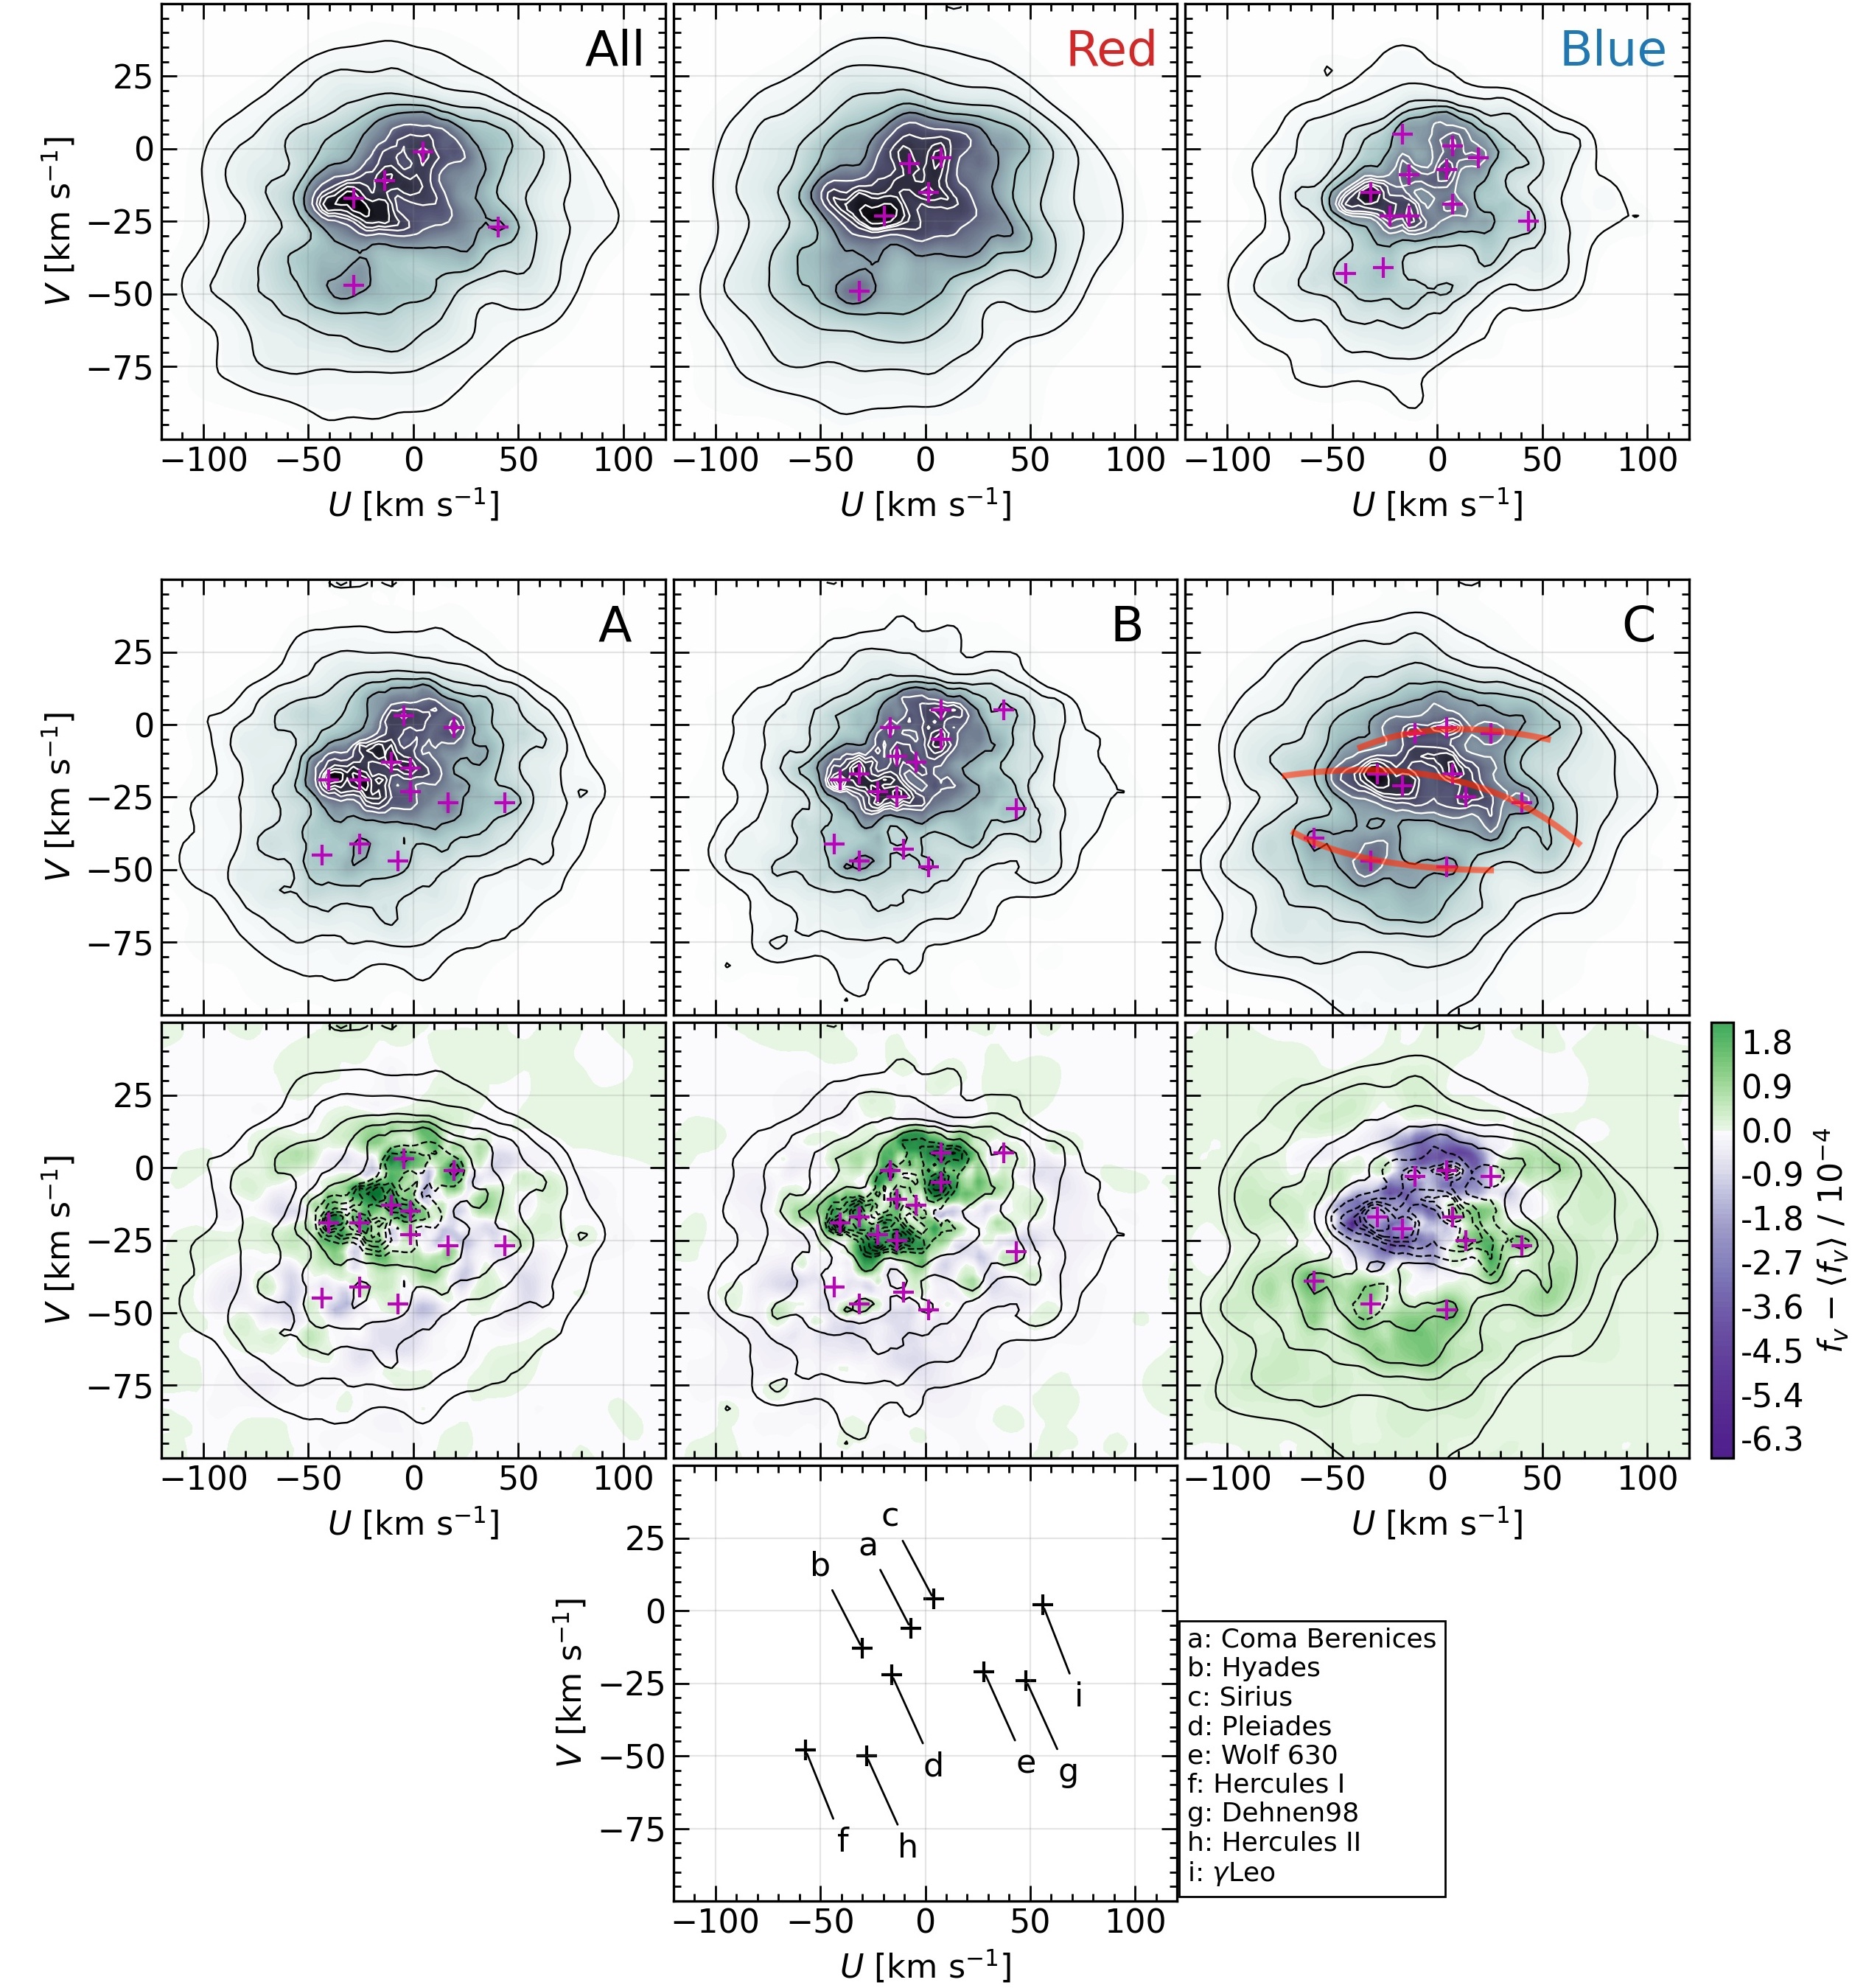
\includegraphics[width=1\textwidth]{images/wds_fv.jpg}
    \caption{Velocity distributions of the WDs in the $U-V$ plane. Purple crosses show identified features. Shown also are the different sub-samples with the top row showing the different bifurcated sequences, the middle row shows the magnitude bins mentioned in section \ref{sec:p2-inferring}. The bottom row shows the distribution of the same magnitude bins subtracted by the mean of the three distributions, to highlight where each bin is strongest or weakest. At the bottom is shown the first nine groups identified in \cite{antoja:12} for comparison.} % Fig. 4.2
    \label{fig:wd_fv}
\end{figure}

We split the WD sample along the bifurcation in the colour-magnitude diagram (between 12th and 14th magnitude where it is strongest) as well as into three equally sized magnitude bins, which we simply call \textit{A}, \textit{B}, and \textit{C} from brightest to faintest. The resulting velocity distributions in $(U, V)$ are seen in Fig. \ref{fig:wd_fv}. While the other velocity projections are also calculated (and shown in the paper) the $(U, V)$ space shows the most structure. The overall shape can be quickly identified to match well with the known distribution of the main-sequence stars as seen in Fig. \ref{fig:veldist}. The magnitude bins can be seen increasing in velocity dispersion as they go from \textit{A} to \textit{C}, reflecting the age-dispersion relation. As the dispersion becomes larger, \textit{C} appears to have arch-like features as well, marked in the plot with red lines. The relative distributions on the third row has an unexpected result. We naturally would expect the more centrally fixated samples \textit{A} and \textit{B} to dominated close to the origin and \textit{C} would dominate further out. This is mostly the case apart from a small region around $(U, V) \approx (7, -19)\ \mathrm{km\ s}^{-1}$. The region does not match conclusively with any known moving group and only \cite{kushniruk:17} provides a nearby link to \textit{Coma Berenices} which has a suggested dynamical origin from a pericenter passing of the \textit{Sagittarius} dwarf galaxy in \cite{monari:18}. 

The regions either side of the CMD bifurcation are seen in the top row and show similar dynamical features. However, the velocity dispersion of the red sample is clearly larger than the blue. This hints of hotter kinematics and as such, we look to the dispersion of the samples rather than the full distribution for further analysis. 
\section{Two kinematic populations}\label{sec:p2-populations}
\begin{figure}[t]
    \centering
    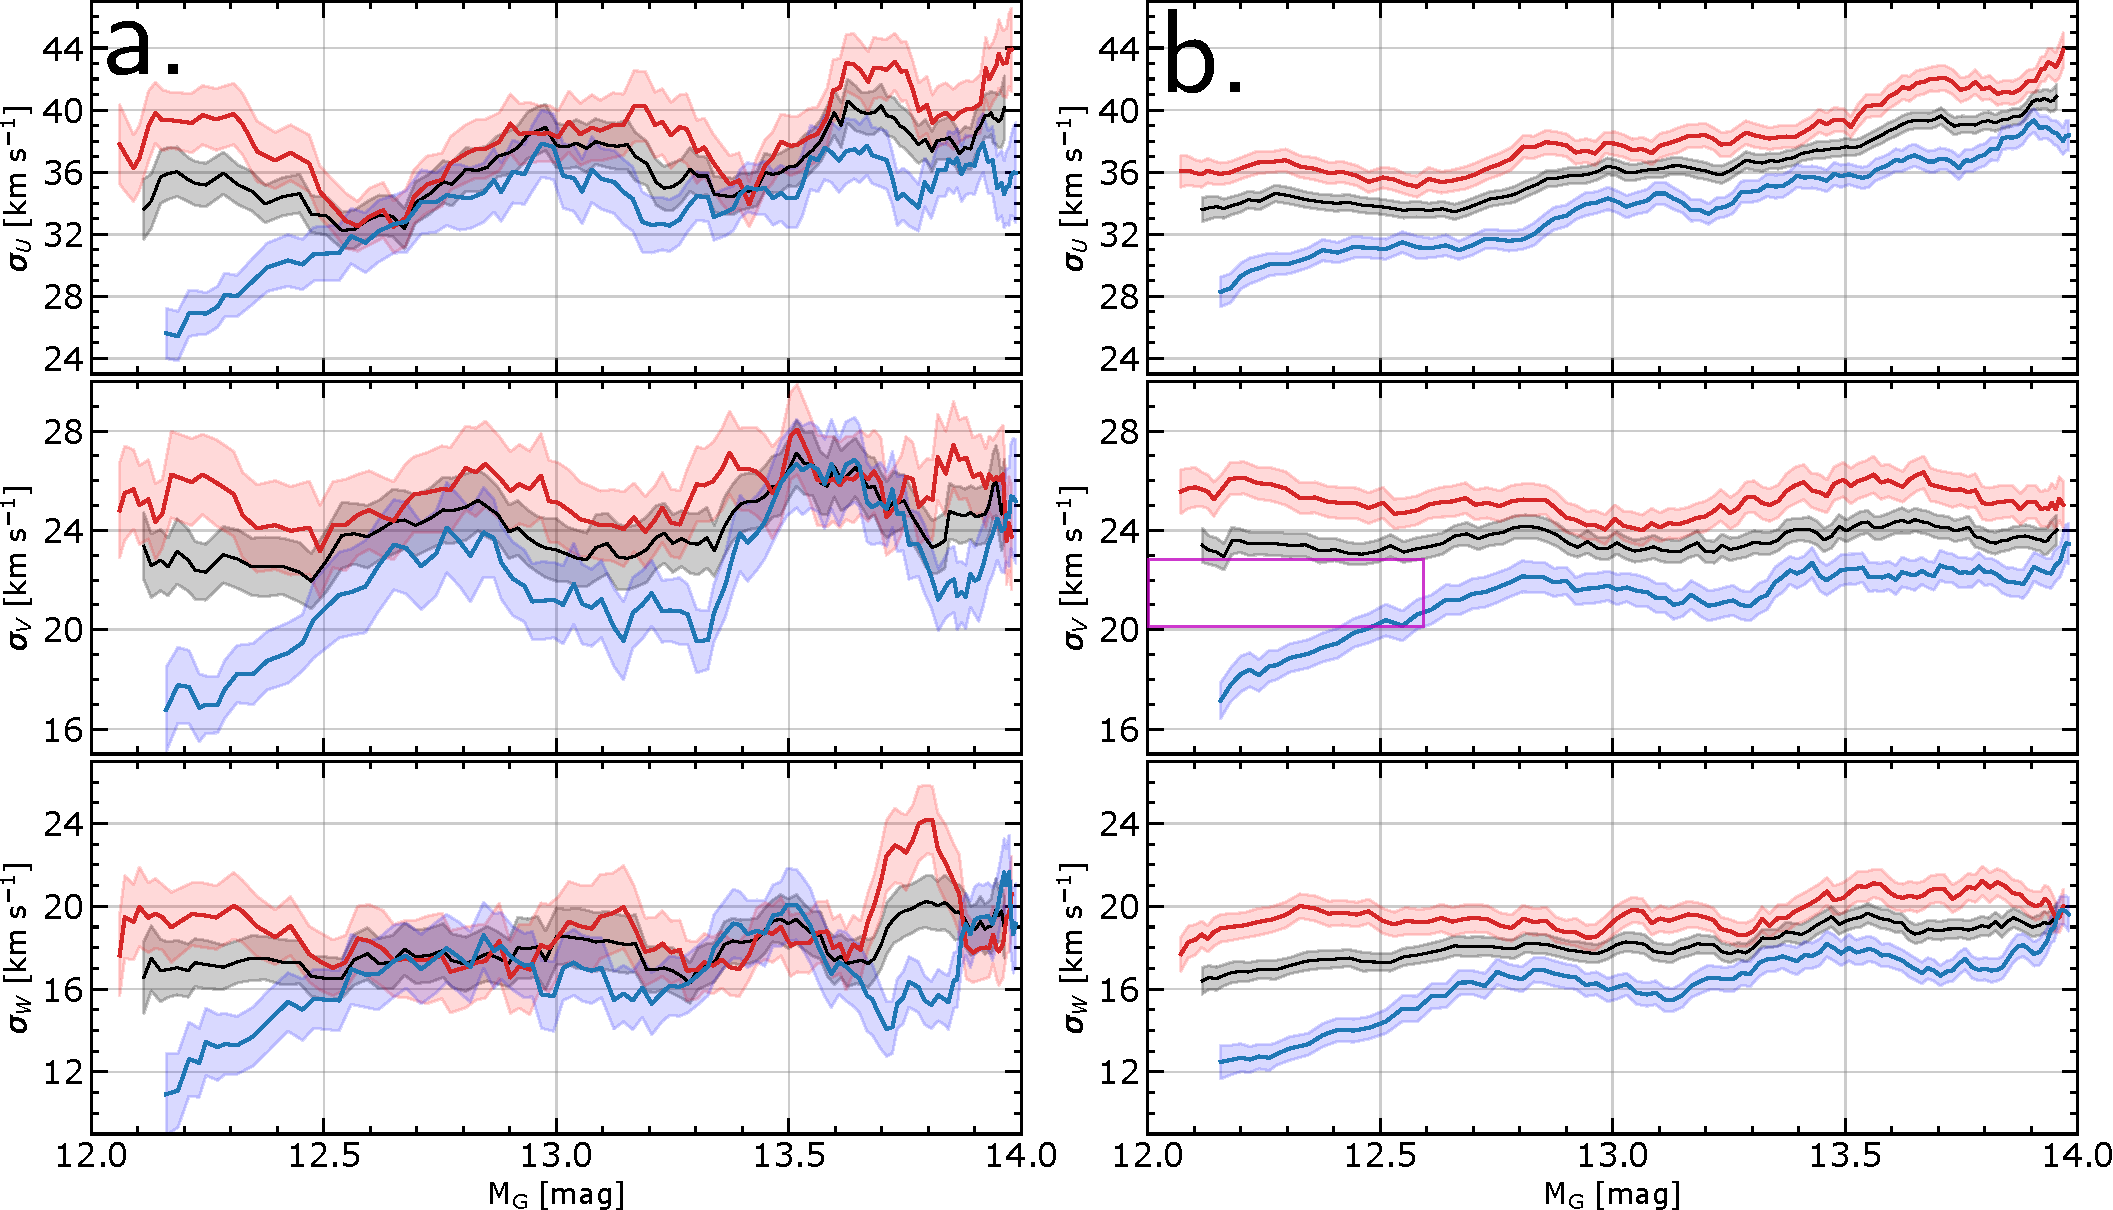
\includegraphics[width=1\textwidth]{images/moving_dispersion.pdf}
    \caption{Moving velocity dispersion calculated in the three directions of $U$, $V$, and $W$, for the bifurcated sequences between 12th and 14th magnitude where they are visible. \textit{a.} shows the moving dispersion for the red and blue sequences as well as the joint sample using WDs which are closer than 100 pc. The shaded regions show the 1$\sigma$ uncertainty regions. \textit{b.} same as the a. but for WDs up to 200 pc. Both plots show clearly a separation between the red and blue samples and when the 200 pc sample is used, they barely even overlap within 1$\sigma$.} % Fig. 4.3
    \label{fig:moving_disp}
\end{figure}
We use the same method as in \cite{dehnen:98b} to determine the velocity dispersion for a sample of stars. But we also employ a moving window across the CMD bifurcation to better compare the sequences as they cool. The velocity distributions shown in Fig. \ref{fig:wd_fv} were found for WDs within 500 pc, whereas here we use WDs limited to either 100 pc or 200 pc, the result of which can be seen in Fig. \ref{fig:moving_disp}. Here it can be clearly seen for the 200 pc sample that the red sequence has a higher velocity dispersion across all magnitudes. For the 100 pc sample this is also visible but less so. We can however show that the two samples are drawn from the same underlying distribution. We determine the following $Q$-statistic for the two dispersion of the samples at various points: 
\begin{equation}
    Q = \frac{\sigma_{d_1} - \sigma_{d_2}}{\sqrt{\Delta \sigma_{d_1}^2 + \Delta \sigma_{d_2}^2}},
\end{equation}
where $d_1$ is the 100 pc sample and $d_2$ are stars between 100-200 pc. Both the red and blue Cumulative Distribution Functions (CDF) match well with a Gaussian distribution, and using a Kolmogorov-Smirnov test gives $P$-values between them and a true Gaussian which all lie above 0.8. Therefore, the difference between the two figures is consistent with simple statistical noise. 

This shows that the two sequences between magnitudes 12 and 14 are \textit{kinematically separate and distinct populations}. In regards to the discussion in section \ref{sec:p2-whitedwarfs}, this would agree neatly with the two sequences being comprised of WDs different masses where the heavier WDs are formed recently, giving them less time to be heated dynamically and thus forming the blue sample we have seen here. It cannot be ruled out the atmospheric composition is partly responsible for the bifurcation in the CMD but it cannot be the sole explanation. In our 100 pc samples, we cross-matched with the Montreal White Dwarf Database \citep{dufour:17} to find that 85\% of the cross-matched red sample and 39\% of the blue are DAs, so there are undoubtedly non-DAs in the second sequence. If they truly correspond to 60\%, they still do not significantly alter the kinematics of the sample as a whole. It can be argued that the crystallization of massive WDs would provide massive WDs which are still visible in our range due to cooling delays (e.g., \citealt{tremblay:19, bergeron:19, bauer:20}). If this were the case, these massive WDs would have been around for long enough to have significant dynamical heating. If this process is contaminating the sample, the fact that we still see the kinematic split is arguably even more significant.

Further insight into the CMD bifurcation of the WD sequence will likely require a combination of both spectroscopic and kinematic study. Here, we have demonstrated the possibilities of working with only proper motions when analysing the vast Gaia datasets. 